% ============================================================
% Section 5.1: EOG Signal Acquisition and Processing Results
% ============================================================
\section{EOG Signal Acquisition and Processing Results}
\label{sec:results_eog_signal}

\subsection{Subject Demographics and Testing Protocol}
\label{subsec:subject_demographics_testing_protocol}

The experimental validation of the integrated platform was conducted involving five healthy male participants (comprising the project engineering team), with an age range of 22--24 years. Due to standard clinical access constraints and the prototype stage of the hardware, testing on actual patients with Locked-in Syndrome (LIS) or severe quadriplegia was deferred to future clinical phases. Testing was conducted in a controlled indoor laboratory environment. To evaluate the impact of the neuromuscular learning curve, the testing protocol intentionally restricted the pre-test training time for the majority of participants. However, one participant (Subject 3) underwent an extended acclimatization session to establish an optimal performance baseline for an experienced user.

\FloatBarrier
\subsection{EOG Waveform Acquisition and Digital Processing Pipeline}
\label{subsec:eog_acquisition_processing_pipeline}

To test the system under real conditions, live experiments were conducted using the setup shown in Figure \ref{fig:experimental_test_setup}. Surface Ag/AgCl electrodes were placed around the user's eyes to capture corneo-retinal biopotentials. The signals were passed through the analog front-end circuit and sent to the processing unit.

\begin{figure}[H]
  \centering
  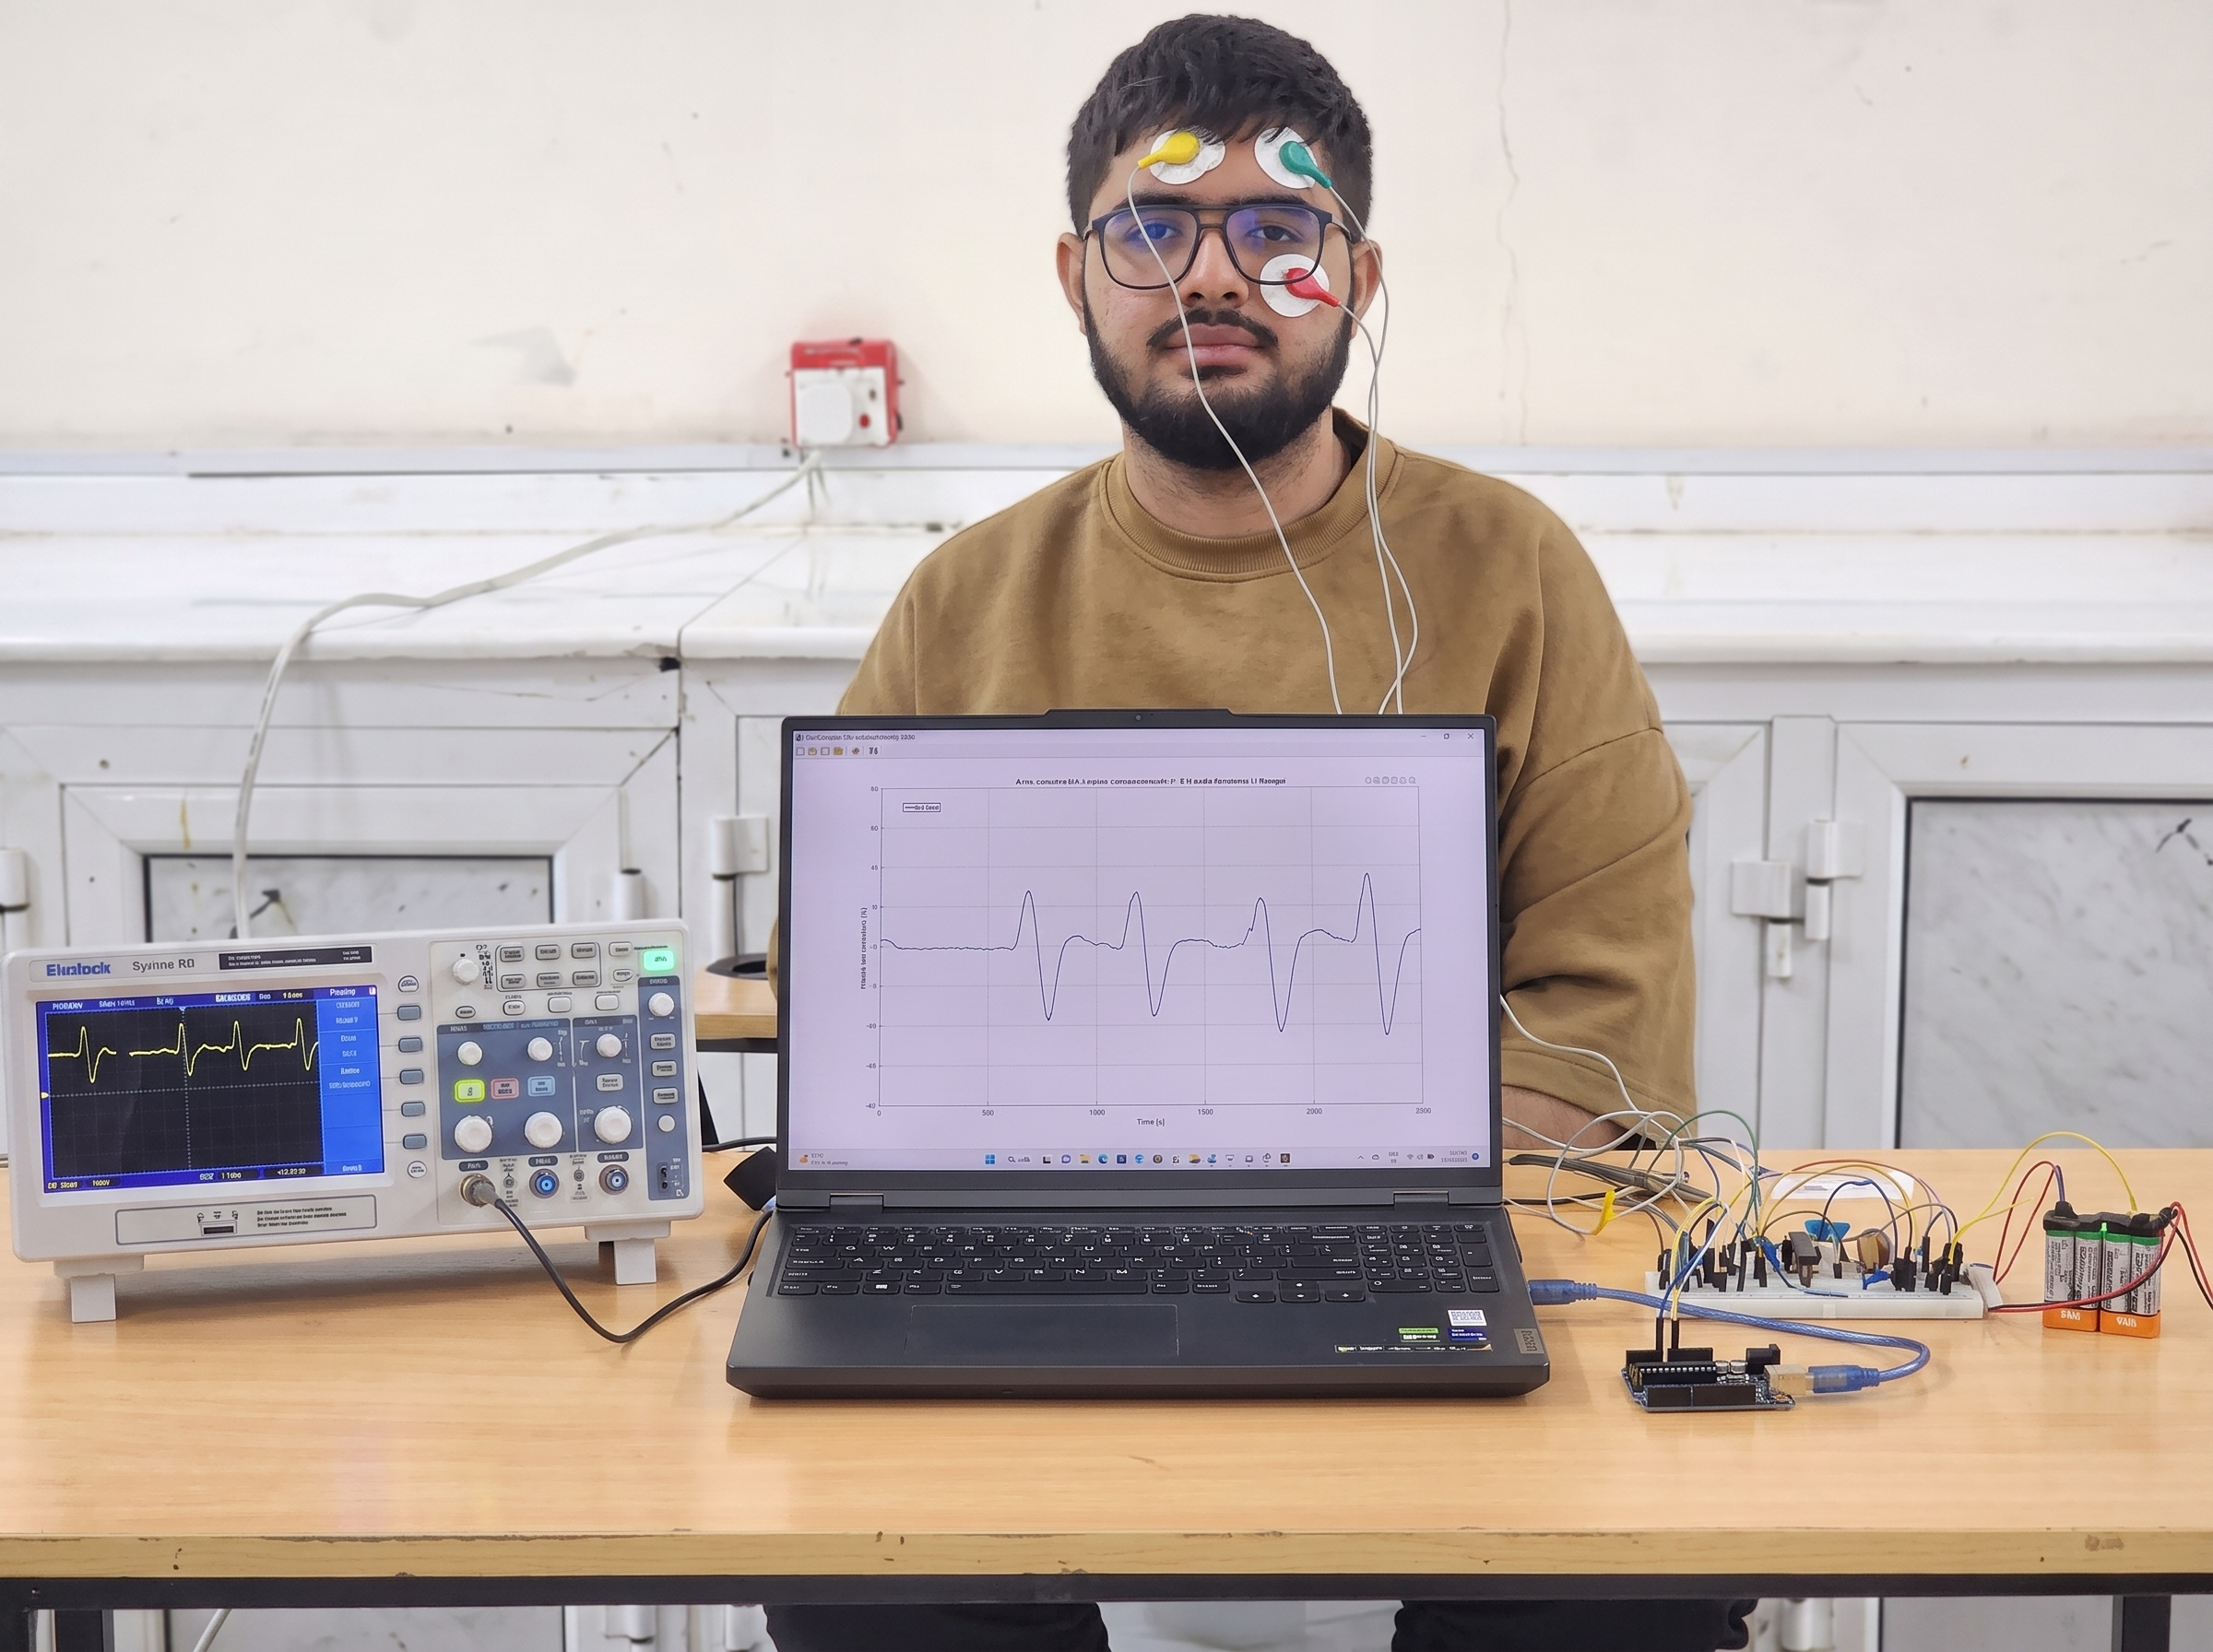
\includegraphics[width=0.85\textwidth]{03_Figures/Ch5/fill_setupp.jpeg}
  \caption{Experimental test setup.}
  \label{fig:experimental_test_setup}
\end{figure}

Acquiring clear EOG signals is challenging because raw biopotentials have microvolt-level amplitudes. The primary AD620 instrumentation amplifier successfully amplified the signal. Figure \ref{fig:raw_eog_oscilloscope_50hz} shows the raw EOG waveform on an oscilloscope. Voluntary blink peaks are visible, but the baseline contains thick noise caused by $50\,\text{Hz}$ power-line interference. This noise confirmed the need for digital filtering.

\begin{figure}[H]
  \centering
  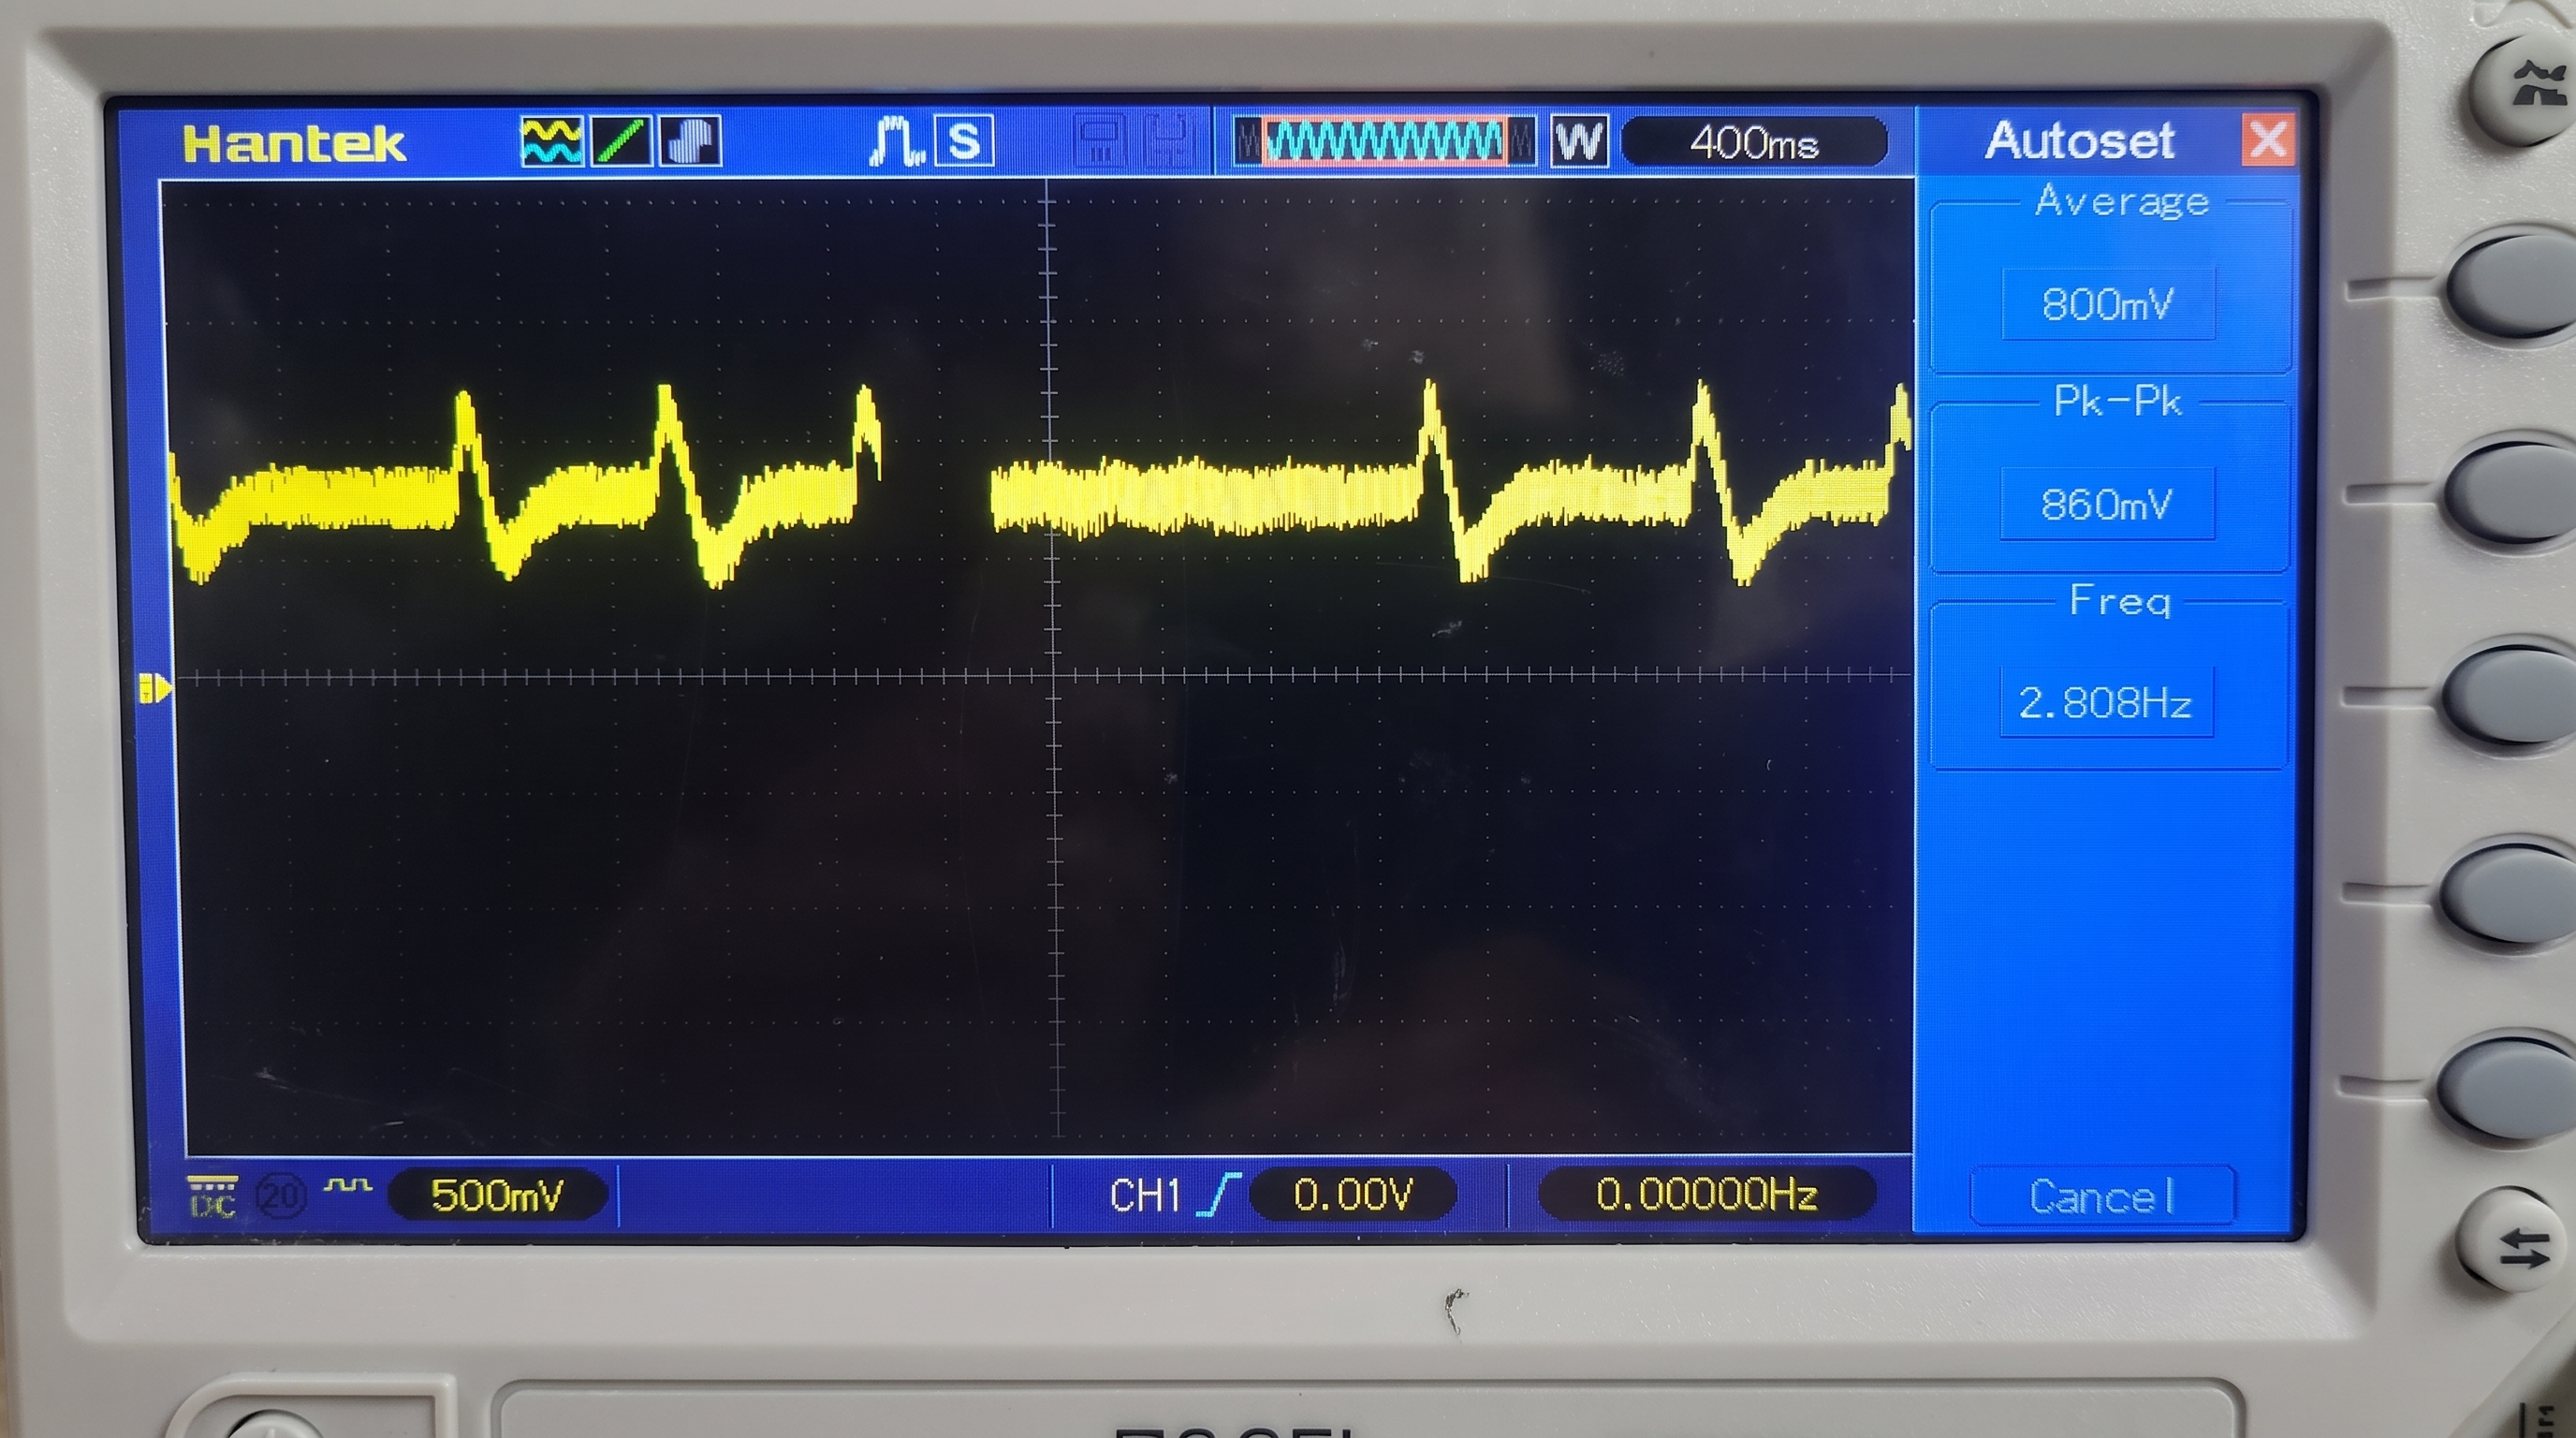
\includegraphics[width=0.85\textwidth]{03_Figures/Ch5/raw_eog_oscilloscope_50hz.jpeg}
  \caption{Raw EOG waveform on oscilloscope.}
  \label{fig:raw_eog_oscilloscope_50hz}
\end{figure}

To remove this interference, the signal was sampled at $250\,\text{Hz}$ using an Arduino microcontroller and transmitted to MATLAB. In MATLAB, the signal was processed using DC offset removal, a digital $50\,\text{Hz}$ notch filter, and a moving average filter to smooth the waveform.

Figure \ref{fig:processed_eog_matlab_thresholds} shows the final processed signal in MATLAB. The baseline noise was removed, allowing the algorithm to set clear threshold lines (dashed lines) for blink detection. This processing pipeline successfully converted the raw eye signals into stable control pulses while preventing false detections.

\begin{figure}[H]
  \centering
  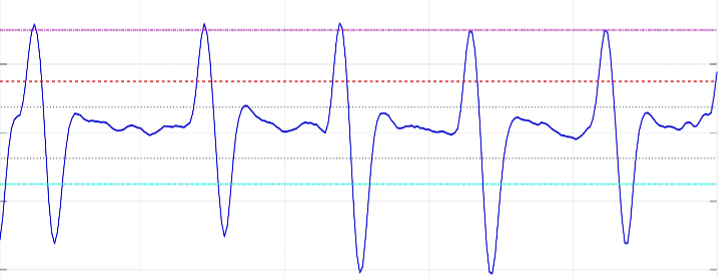
\includegraphics[width=0.85\textwidth]{03_Figures/Ch5/processed_eog_matlab_thresholds.png}
  \caption{Processed EOG signal in MATLAB.}
  \label{fig:processed_eog_matlab_thresholds}
\end{figure}
